

    \item A point charge \( +Q \) is placed just outside an imaginary hemispherical surface of radius \( R \) as shown in the figure. Which of the following statements is/are correct?
        \begin{tasks}(1)
            \task The electric flux passing through the \textit{curved} surface of the hemisphere is \(- \frac{Q}{2\varepsilon_0} \left( 1 - \frac{1}{\sqrt{2}} \right)\)
            \task Total flux through the curved and the flat surfaces is \(\frac{Q}{\varepsilon_0}\)
            \task The component of the electric field normal to the flat surface is constant over the surface
            \task The circumference of the flat surface is an equipotential
        \end{tasks}


\begin{center}
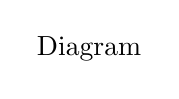
\begin{tikzpicture}
\node {Diagram};
\end{tikzpicture}
\end{center}
